\documentclass{acm_proc_article-sp}
\usepackage{float}
\begin{document}

% --- Author Metadata ---
% Note: The \date command is ignored by this class
\title{AI201 PA 2 Report\\ Naive Bayes Spam Filter}

\numberofauthors{1}
\author{
\alignauthor Micko Adrian M. Miradora (2025-22234)\\ 
~\\
Date of Submission: March 11, 2026
}

\maketitle

\section{Introduction}
Spam detection is a two-category classification problem in which emails are categorized as legitimate messages (ham) or unsolicited messages(spam). Although early filters relied on knowledge engineering and hand-crafted rules, modern approaches utilize supervised machine learning to create filters optimized for an individual user's email distribution. This report presents a Naive Bayes spam filter utilizing class conditional likelihood and feature selection techniques, specifically Mutual Information and frequency filtering, based on the methodologies by Hovold (2005).

To optimize classification performance, this implementation addresses the challenges of limited data through Lambda smoothing, which modifies the class conditional likelihoods to prevent zero-probability errors for unseen words. Furthermore, to prevent rounding to zero during the product notation of the Naive Bayes classifier, all calculations are performed in the logarithmic domain. Additionally, the denominator was removed from the Naive Bayes classifier calculation because it acts as a constant scaling factor for both the spam and ham classes. Since the objective is strictly classification, computing this identical denominator for both sides is mathematically redundant and computationally inefficient.

A focus of this report is the evaluation of Hovold’s Mutual Information technique to identify the most discriminative attributes within the TREC06 corpus. A frequency filter is utilized as a pre-processing step to prune the top non-informative words, which prevents common vocabulary, specifically stopwords, from dominating the total vocabulary size. By comparing the classifier's performance across varying smoothing parameters, restricted vocabulary sizes (specifically the top 200 and 400 features) and frequency filter, this report analyzes the trade-offs between computational efficiency and the model's ability to maintain high recall.



\section{Objectives} The primary objectives of this study are:
\begin{itemize}
    \item To construct a custom Naive Bayes classifier from scratch using Python without using external Bayesian libraries.
    \item To evaluate the impact of Lambda Smoothing on handling zero probabilities for words not present in the training data.
    \item To optimize the classifier using Hovold's Mutual Information to identify the top 200 most informative words.
    \item To measure performance through precision and recall.
\end{itemize}

\section{Methodology}
The methodology for this spam filter is structured around a Naive Bayes implementation utilizing boolean attribute representation, class conditional likelihood, lambda smoothing, frequency filtering, hovold's mutual information and evaluation functions. 

\subsection{Data Retrieval, Preprocessing and Partitioning}
The dataset used for this report is a subset of the TREC06p Public Spam Corpus. The data was first retrieved and partitioned into two disjoint sets: a Training Set (70\%) and a Test Set (30\%). This partition was randomized using a fixed seed (random.seed(42)) for the reproducibility of the results in different experimental runs.

Following partition, each email document was parsed using a custom tokenizer. Based on the assignment requirements, a "word" was defined as any sequence of alphabetic characters [a-zA-Z] delimited by whitespace, with optional trailing commas or periods removed. Case sensitivity was preserved to capture distinct typography in aggressive spam. Afterwards, the  tokens for each document were added to a unique set.

\subsection{Model Training}
The variables needed for classification are established during the initial training phase, which processes the randomized 70\% training partition. For each email, the system extracts the parsed tokens and adds it to a unique set. Afterwards, it increments the occurrence of a token within their respective class dictionary only once per document, regardless of the token's total amount within the email.

Additionally, this training function calculates the prior probability $P(C)$ for both the spam and ham categories based on their relative distributions within the training subset. The training algorithm also calculates the document frequency for each word $x_i$. This is achieved by maintaining two primary counters for cardinality $|D_{\omega}|$ and summation of indicator function $\sum_{D\in D_{\omega}}I(x_i\in D)$. Lastly, the system creates a master vocabulary by collecting all the unique words found throughout the training emails. 

\subsection{Class Conditional Likelihood and Lambda Smoothing}
The system calculates the class conditional likelihood $P(x_i|\omega)$ which is the probability that a word $x_i$ appears in a document given that the document belongs to class $\omega$ (spam or ham). However, real-world textual data often presents the "zero-frequency problem," where valid tokens present in the test set may be absent from the training vocabulary. 

A single zero-probability would result in a 0 for the entire probability product. To resolve this, the implementation utilized Lambda smoothing into the get\_word\_percentage function. This technique adjusts the likelihood by adding a small smoothing parameter $\lambda$ to the frequency counts. The class conditional likelihood is defined as:
$$P(x_{i}|\omega)=\frac{[\sum_{D\in D_{\omega}}I(x_{i}\in D)]+\lambda}{|D_{\omega}|+\lambda|V|}$$
where $|V|$ is the vocabulary size and $I(\cdot)$ is an indicator function representing the presence of a word in a document class.

It computes the class conditional likelihood by retrieving the training documents that contained the word, and dividing it by the total number of documents in that class. Additionally, this function utilizes lambda smoothing. Before division, it adds the small $\lambda$ value to the word counts to prevent 0 products.

Afterwards, a test was conducted to find the optimal smoothing factor using the lambda\_smoothing function. The classifier was evaluated using five $\lambda$ values: $\{2.0, 1.0, 0.5, 0.1, 0.005\}$. For each $\lambda$, the function temporarily updates the classifier's configuration and processes the entire test set. Performance was measured using F1 Score to find the best balance between Precision and Recall. 

\subsection{Naive Bayes Algorithm}
 A Naive Bayes classifier was implemented without the usage of external machine learning libraries using the classify function. The classifier estimates the probability of a class $\omega$ (Spam or Ham) given a document $D$ using Bayes' Theorem:
$$P(\omega | x_1, x_2, \dots, x_d) = \frac{\prod_{i=1}^{d} P(x_i | \omega) P(\omega)}{\sum_{\omega} \prod_{i=1}^{d} P(x_i | \omega) P(\omega)}$$

To prevent rounding to zero caused by multiplying many small probabilities, all calculations were performed in log-space. The final classification decision was made by comparing the converted logarithm probabilities:
$$\log P(\omega) + \sum \log P(x_i | \omega)$$

The classifier begins by setting the baseline scores using the prior probabilities, $\log P(\text{spam})$ and $\log P(\text{ham})$, which were calculated during training. It then loops through each word in the email, using the get\_word\_percentage function to find the probability of that specific word. Finally, the system adds up all the log probabilities for both classes. 

\subsection{Hovold's Feature Selection and Frequency Filtering}
The system implements Hovold’s Mutual Information (MI) to optimize the words utilized by the model and filter out uninformative noise using hovold\_mutual\_information function. Rather than forcing the Naive Bayes function to process the entire vocabulary, this method evaluates how effectively each specific word discriminates between the spam and ham classes. For every word in the vocabulary, the MI score was calculated based on the four possible states: Present in Spam, Present in Ham, Absent in Spam, Absent in Ham.
$$\sum_{x \in \{0, 1\}} \sum_{c \in C} P(x, c) \log \frac{P(x, c)}{P(x)P(c)}}$$

Words were ranked by their MI score, and the model was re-evaluated using restricted vocabularies of the Top 200 and 400 features to assess the trade-off between computational efficiency and recall. 

To evaluate the impact of non-informative words on model performance, frequency filtering is implemented using the remove\_most\_frequent\_words function. This preprocessing step identifies and eliminates the highest-occurring words across the dataset. Because these terms, often English stopwords like "the" or "and", appear heavily in both spam and ham emails, they provide minimal predictive value. By testing the classifier both with and without this filter, the experiment assesses whether removing these high-frequency terms improves classification accuracy and reduces computational overhead.

\subsection{Performance Metrics}
The classifier's performance was evaluated using Precision and Recall. A Confusion Matrix was generated for each experimental stage to visually analyze the distribution of True Positives, False Positives, True Negatives, and False Negatives

\subsection{Main Execution}
The system is executed by a main function that links data processing, model training, classifying, class likelihood condition, frequency filter, mutual information, plotting and performance evaluation. Initially, the dataset is retrieved, parsed, and partitioned into distinct training and testing subsets The Naive Bayes classifier is instantiated and trained on the training subset to construct the initial model and the baseline vocabulary and calculate initial prior probabilities. 

Afterwards, the function calls the lambda\_smoothing function to identify and apply the optimal $\lambda$ parameter. To assess the optimizations, the script conducts classification experiments. First, it isolates the top 200 and 400 most informative terms using the hovold\_mutual\_information metric and evaluates the resulting performance. Subsequently, it introduces the remove\_most\_frequent\_words filter to eliminate the 200 most informative terms before recalculating the optimal Mutual Information feature sets.  Throughout these progressive phases, the system continuously classifies the test documents and generates Precision and Recall metrics alongside confusion matrices.

\section{Experimental Results}
The classifier was tested with five values of $\lambda$ to find the optimal balance between precision and recall.

\begin{table}[H]
\centering
\caption{Smoothing Results on TREC06 Subset}
\begin{tabular}{|c|c|c|c|}
\hline
$\lambda$ Value & Precision & Recall & F1-Score\\ \hline
2.0 & 0.9931 & 0.9841 & 0.9886\\ \hline
1.0 & 0.9945 & 0.9813 & 0.9879\\ \hline
0.5 & 0.9962 & 0.9757 & 0.9858\\ \hline
0.1 & 0.9983 & 0.9475 & 0.9722\\ \hline
0.005 & 0.9997 & 0.9205 & 0.9585\\ \hline
\end{tabular}
\end{table}

Lower values of $\lambda$ (e.g., 0.005) resulted in the highest Precision (0.9997) but the lowest Recall (0.9205).  As $\lambda$ increased, the model became better at generalizing, significantly improving Recall. The experiment identified $\lambda = 2.0$ as the optimal value by achieving the highest F1 Score of 0.9886.

\begin{figure}[H]
    \centering
    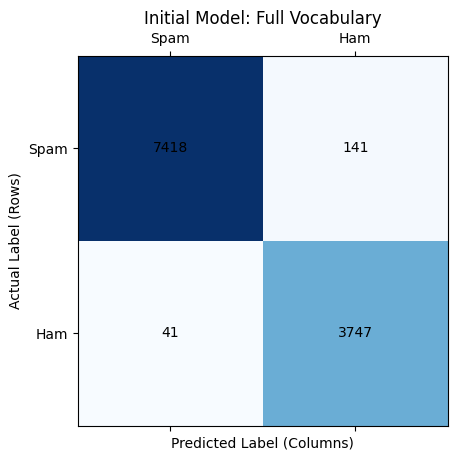
\includegraphics[width=0.6\linewidth]{Initial_Model.png}
    \caption{Initial Model (Lambda = 1)}
    \label{fig:placeholder}
    \vspace{-0.5 cm}
\end{figure}

The initial model used the entire vocabulary and a default smoothing value of 1.0. It correctly identified 7,418 spam and 3,747 ham emails. It  missed 141 spam emails (False Negatives) and incorrectly flagged 41 ham emails as spam (False Positives). It has a precision of 0.9945 and recall of 0.9813.

\begin{figure}[H]
    \centering
    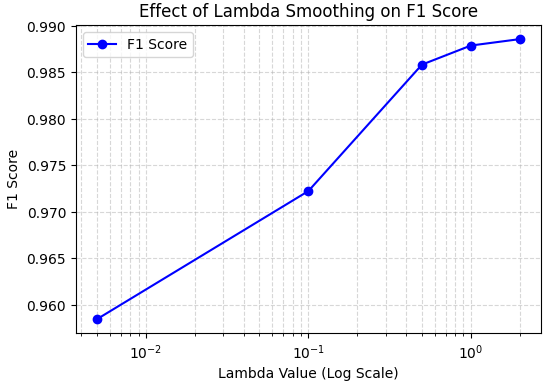
\includegraphics[width=0.75\linewidth]{Lambda_Smoothing_F1_Score.png}
    \caption{Lambda Smoothing F1 Score}
    \label{fig:placeholder}
    \vspace{-0.5 cm}
\end{figure}

To find the best settings, the system tested five different $\lambda$ values. As shown in the "Effect of Lambda Smoothing on F1 Score" graph, the F1-Score steadily improved as the $\lambda$ value increased. The model reached its peak performance at $\lambda = 2.0$. 

\begin{figure}[H]
    \centering
    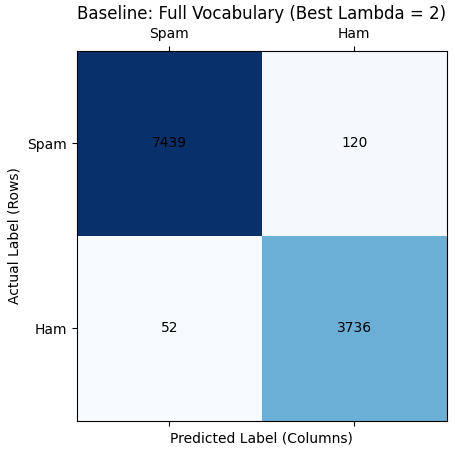
\includegraphics[width=0.6\linewidth]{Baseline_Model_Best_Lambda.png}
    \caption{Baseline Model (Lambda = 2)}
    \label{fig:placeholder}
    \vspace{-1 cm}
\end{figure}

The highest classification score was achieved using the full vocabulary with an optimized smoothing parameter of $\lambda = 2.0$. Under this configuration, the model correctly identified 7,439 spam emails and 3,736 ham emails. By fine-tuning the $\lambda$ value, the system reduced missed spam (False Negatives) from 141 down to 120. It has a precision of 0.9931 and recall of 0.9841.

\begin{figure}[H]
    \centering
    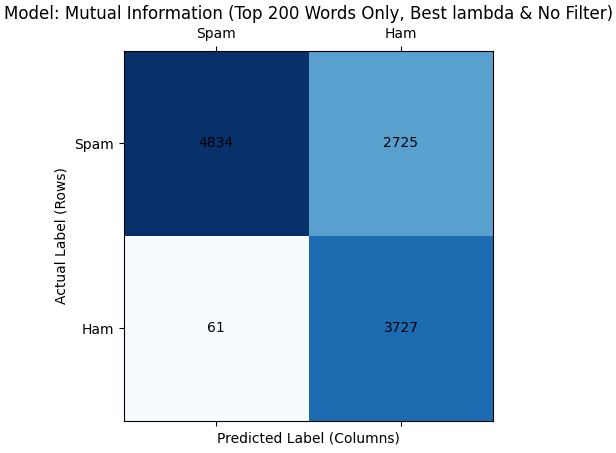
\includegraphics[width=0.8\linewidth]{Model_MI_200_NoFilter.png}
    \caption{Mutual Information Model with 200 Vocabulary Size}
    \label{fig:placeholder}
    \vspace{-0.75 cm}
\end{figure}

Implementing Hovold's Mutual Information to compress the feature space resulted in a significant drop in recall. When restricted to only the Top 200 most informative words, the classifier underperformed, misclassifying 2,725 spam emails as ham. It has a precision of 0.9875 and recall of 0.6395.

\begin{figure}[H]
    \centering
    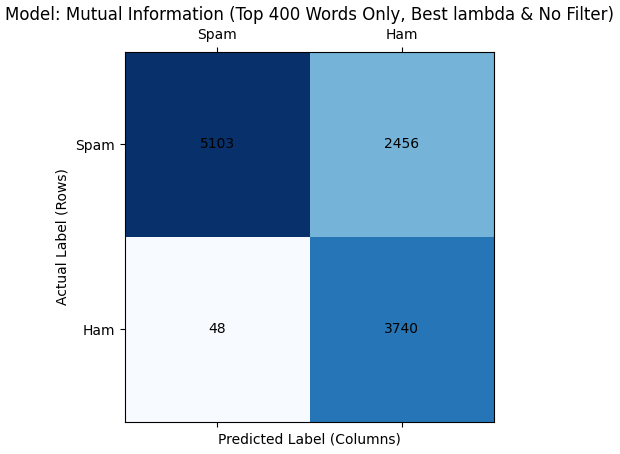
\includegraphics[width=0.8\linewidth]{Model_MI_400_NoFilter.png}
    \caption{Mutual Information Model with 400 Vocabulary Size}
    \label{fig:placeholder}
\end{figure}

Expanding the feature space to the Top 400 words provided a marginal improvement by reducing false negatives to 2,456. However, the high error indicated that the Mutual Information was capturing too much "noise" when applied to an unfiltered vocabulary. It has a precision of 0.9907 and recall of 0.6751.

\begin{figure}[H]
    \centering
    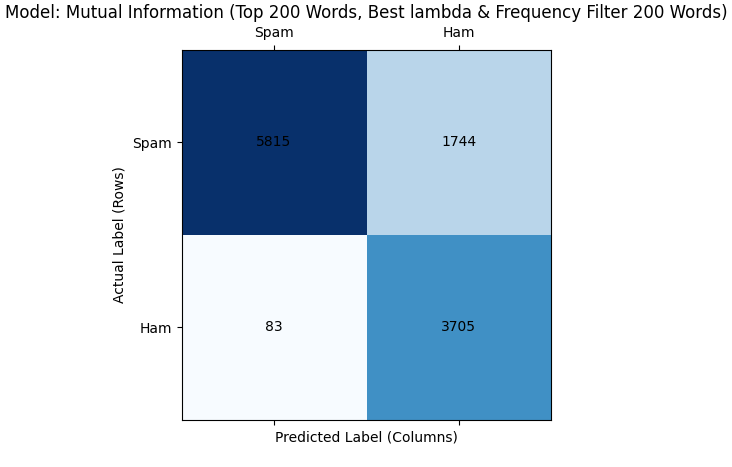
\includegraphics[width=0.9\linewidth]{Model_MI_200_WithFilter.png}
    \caption{Mutual Information Model with 200 Vo-
cabulary Size and Frequency Filter}
    \label{fig:placeholder}
    \vspace{-0.5 cm}
\end{figure}

To address the noise captured by the initial MI ranking, the remove\_most\_frequent\_words filter was applied prior to recalculating the MI scores. Removing the 200 most informative words from the corpus yielded improvements across the  models. The filtered Top 200 model saw false negatives plummet from 2,725 down to 1,744. It has a precision of 0.9859 and recall of 0.7693.

\begin{figure}[H]
    \centering
    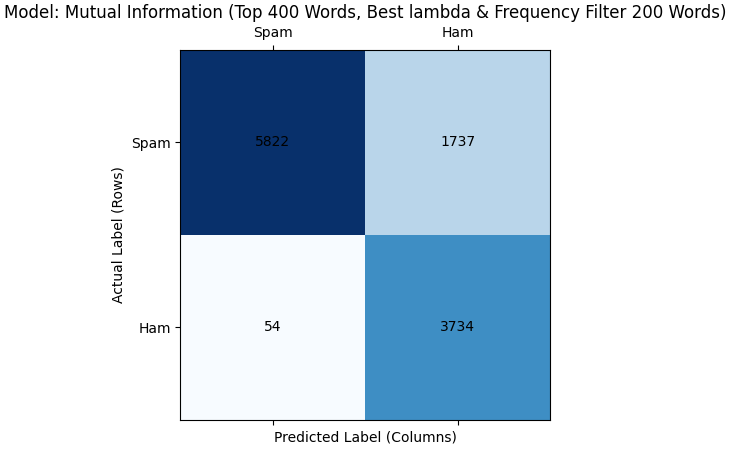
\includegraphics[width=0.9\linewidth]{Model_MI_400_WithFilter.png}
    \caption{Mutual Information Model with 400 Vo-
cabulary Size and Frequency Filter}
    \label{fig:placeholder}
    \vspace{-0.5 cm}
\end{figure}

The Top 400 model paired with the frequency filter achieved the strongest performance among all the reduced vocabulary size experiments. It identified 5,822 spam emails and 3,734 ham emails, yielding only 54 false positives. While the restricted vocabularies could not match the  accuracy of the 50,000+ word baseline, these results prove that stripping high-frequency stopwords is a mandatory step to preserve classification accuracy when optimizing for computational efficiency. It has a precision of 0.9908 and recall of 0.7702.

\section{Analysis and Discussion of Results}
The experimental results demonstrated the effectiveness of a custom-built Naive Bayes classifier in distinguishing between spam and ham within the TREC06 corpus. A primary observation from the initial stages of the experiment is the importance of probability smoothing in handling zero frequency tokens, where valid tokens present in the test set are absent from the training data. As the smoothing parameter $\lambda$ was increased from 0.005 to 2.0, the model's recall improved significantly from 0.9205 to 0.9841. This indicated that higher smoothing values allow the model to generalize more effectively to unseen vocabulary. While lower $\lambda$ values, such as 0.005, yielded the highest overall precision at 0.9997, which proved ineffective for real-world application by missing a larger amount of spam messages. The highest F1-Score of 0.9886 was achieved at $\lambda=2.0$. This optimized configuration reduced the number of missed spam emails (False Negatives) from 141 in the initial model down to 120, while maintaining a precision of 0.9931. Consequently, this established the "upper bound" for classification performance using the full master vocabulary of 99,700 unique words.

From this experiment, the evaluation of Hovold’s Mutual Information as a technique for dimensionality reduction and feature selection was evaluated. The results were ineffective on the mutual information metric when applied to a raw, unfiltered vocabulary. Specifically, when the feature space was restricted to only the top 200 most informative words without prior preprocessing, the classifier’s recall collapsed, misclassifying 2,725 spam emails as ham. This showed that the mutual information calculation was "distracted" by non-informative words, such as "the," "and," or "to", which appear with high frequency across both classes. Furthermore, expanding the feature space to the top 400 words provided only a marginal improvement, with false negatives remaining high at 2,456.

To mitigate this noise, the remove\_most\_frequent\_words function was introduced as a preprocessing step to remove the top 200 most frequent terms. This intervention redirected the MI ranking toward high-signal keywords which resulted in performance increase. Specifically, in the filtered Top 200 MI model, the number of false negatives reduced from 2,725 to 1,744. The Top 400 MI model paired with frequency filtering resulted as the most optimized configuration among the reduced-dimensionality experiments, correctly identifying 5,822 spam emails and 3,734 ham emails while yielding only 54 false positives. While these restricted vocabularies could not match the raw accuracy of the 50,000-word baseline, the results prove that stripping high-frequency stopwords is a mandatory prerequisite for preserving classification accuracy when optimizing for computational efficiency.

\section{Conclusion}
This report demonstrated the construction and evaluation of a custom Naive Bayes spam filter optimized through Hovold’s Mutual Information, frequency filtering and  Lambda smoothing techniques. The primary objective of constructing a functional classifier from scratch was achieved by yielding a baseline that identified 7,439 spam and 3,736 ham emails. 

This report emphasized that while a comprehensive vocabulary provides the most robust classification, it is the strategic calibration of  $\lambda=2.0$—that allows the model to generalize effectively and achieve its peak F1-Score of 0.9886.

The report proved that feature selection is not merely mathematical ranking but needs an understanding of data "noise." Hovold’s Mutual Information alone was insufficient for maintaining high recall when applied to a raw dataset. 

However, the integration of a frequency filter to prune stopwords allowed the model to compress its vocabulary size to just 400 words while maintaining a precision of 0.9908. As a result, this report provided a spam filter framework that balances the trade-offs between computational efficiency and predictive accuracy in real-world email distributions.

\section{References}
\begin{itemize}
    \item [1] Johan Hovold, Naive Bayes Spam Filtering using Word Position Attributes, In Conference on Email and Anti-Spam, Stanford University, 2005.
    \item [2] University of the Philippines, "AI201 Programming Assignment 2 Instructions," Department of Computer Science, 2026.
    \item [3] M. Sahami, S. Dumais, D. Heckerman, and E. Horvitz, "A Bayesian approach to filtering junk e-mail," in AAAI Workshop on Learning for Text Categorization, Madison, WI, 1998, pp. 98-105.
\end{itemize}

\end{document}